\documentclass[class=article, crop=false, 11pt]{standalone}
\usepackage[english]{babel}
\usepackage[utf8]{inputenc}
\usepackage[T1]{fontenc}
\usepackage{float}
\usepackage{lmodern,amsmath,amssymb,amstext,amsfonts,mathrsfs,graphicx,caption}
\usepackage[width=14cm]{geometry}
\usepackage[colorlinks,pdfpagelabels,pdfstartview = FitV,bookmarksnumbered = true, bookmarksopenlevel=section, linkcolor = black,hypertexnames = false,citecolor = black,pdfpagelabels=false, urlcolor=black]{hyperref}
\usepackage{rotating}
\usepackage[nottoc]{tocbibind}
\usepackage{natbib}
\usepackage{pdfpages}

\usepackage{chngcntr} % 			** Damit die Bilder Tabellen und Gleichungen 
\counterwithin{figure}{section}	%	** alle nach Kapiteln nummeriert sind.
\counterwithin{table}{section}%		**
\counterwithin{equation}{section}%	**	


%Preambelteil für Main-File
\usepackage[subpreambles=true]{standalone}
\usepackage{import}

%nocite Neudefinition, damit es mit dem Standalone-Paket funktioniert.
%https://tex.stackexchange.com/questions/102234/problem-when-using-nocite-together-with-the-standalone-package
\makeatletter
\def\@documentnocite#1{\@bsphack
	\@for\@citeb:=#1\do{%
		\edef\@citeb{\expandafter\@firstofone\@citeb}%
		\if@filesw\immediate\write\@auxout{\string\citation{\@citeb}}\fi
		\@ifundefined{b@\@citeb}{\G@refundefinedtrue
			\@latex@warning{Citation `\@citeb' undefined}}{}}%
	\@esphack}
\AtBeginDocument{\let\nocite\@documentnocite}
\makeatother

\begin{document}
	
	\import{sections/}{../CoverSheet}
	% Blankpage without numbering
	\newpage
	\
	\thispagestyle{empty}
	\newpage

	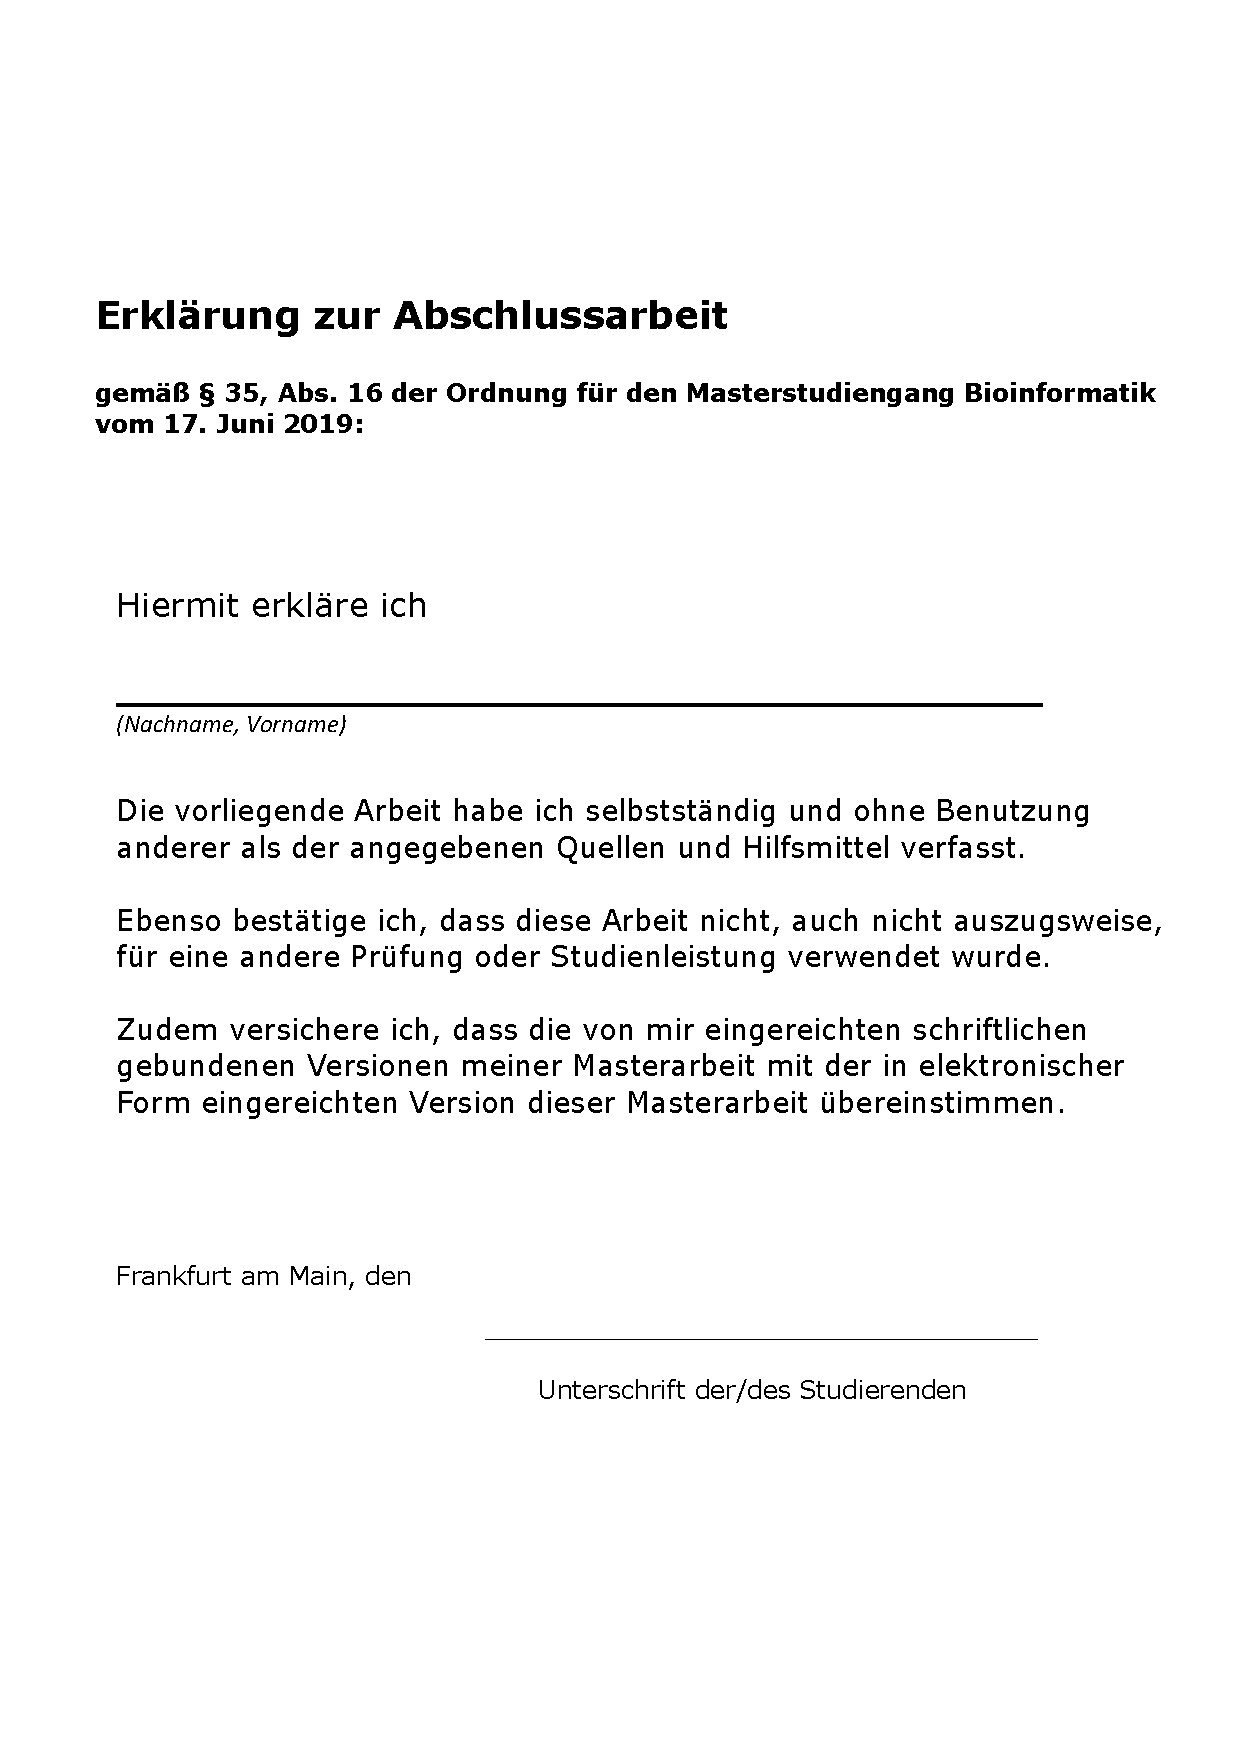
\includepdf[pages=-]{PA_Erklaerung.pdf}

	\newpage
	\
	\thispagestyle{empty}
	\newpage

	\import{sections/}{../Abstract_DE}
	\newpage
	\
	\thispagestyle{empty}
	\newpage

	\import{sections/}{../Abstract_EN}
	\newpage
	\
	\thispagestyle{empty}
	\newpage

	\pagenumbering{roman}
	\pagenumbering{arabic}
	\tableofcontents
	\clearpage

	\import{sections/}{../Introduction}
	\clearpage
	\import{sections/}{../Methods}
	\clearpage
	\import{sections/}{../Results}
	\clearpage
	\import{sections/}{../Discussion}
	\clearpage
	\import{sections/}{../List_of_notations}
	\addcontentsline{toc}{section}{Symbols and Modeling Values}
	\clearpage
	\listoffigures
	\clearpage
	\import{sections/}{../Thanks}
	\addcontentsline{toc}{section}{Acknowledgements}
	\addcontentsline{toc}{section}{Supplementary material}
	\clearpage

	\nocite{*}
	\bibliographystyle{alpha}
	\bibliography{bib}
	
\end{document}